%!TEX root = ../report.tex

\chapter{Experimental Evaluation}

Since the major contribution of this work is the creation of the dataset, the experiments are focused on validating the effectiveness of the dataset. 

% Add visual segmentation masks in all results.

\section{Comparing dataset variants} 

	\begin{itemize}
		\item \textbf{Objective}: The objective of this experiment is to compare the performance of deepLabv3+ on the different dataset variants.
		\item \textbf{Expected result}: DeepLabv3+ is expected to obtain a higher mIOU when the number of classes is lower. This is based on the notion that when similar objects are considered as different classes, the model would not have sufficient features to distinguish them.
		\item \textbf{Inference from the results}: Deeplabv3+ with both the mobileNetv2 network backbone and the Xception network backbone are evaluated on all variants of variety of backgrounds and white backgrounds dataset. From Figure \ref{Fig:vars}, it is evident that the mIOU obtained on each variant is dependent on the properties of objects in the variant. The atWork\_full variant treats all the 18 objects in the dataset as different classes. As a result, for instance, "m20" and "m30" have different labels despite the fact that the two objects only differ in size and slightly in color. The segmentation model is thus forced to distinguish between such objects. Since the objects occur in the dataset at arbitrary scales and are subject to differences in illumination, the real world differences between such similar objects become insignificant in the dataset. Thus, the mIOU obtained on the atWork\_full variant is indeed the lowest as expected. The two variants atWork\_size\_invariant and atWork\_similar\_shapes combine objects which are similar. As a result, deepLabv3+ achieves better mIOU on these variants. The atWork\_binary variant requires the deepLabv3+ to only distinguish foreground from background leading to the highest mIOU. Evidently, the stated inferences are independent of the network backbone used by deepLabv3+. The mIOU values obtained are tabulated in Table \ref{Table:vars}.
	\end{itemize}
	
	\begin{figure}
		\begin{subfigure}{.5\textwidth}
			\centering
			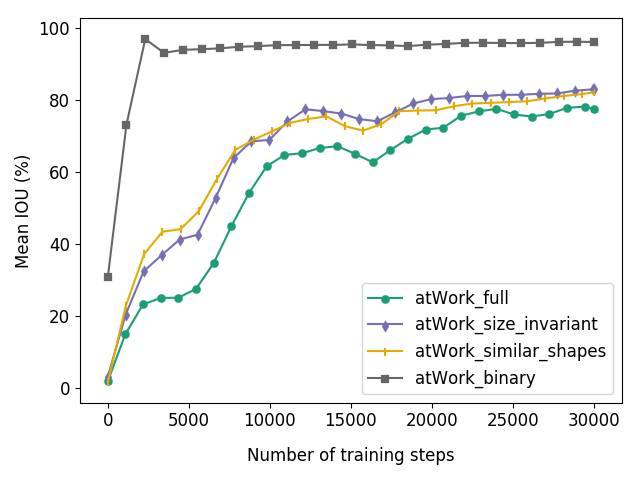
\includegraphics[width=1\linewidth]{images/mobi_4vars}
			\label{Fig:mobivarsa}
			\caption{}
		\end{subfigure}
		\begin{subfigure}{.5\textwidth}
			\centering
			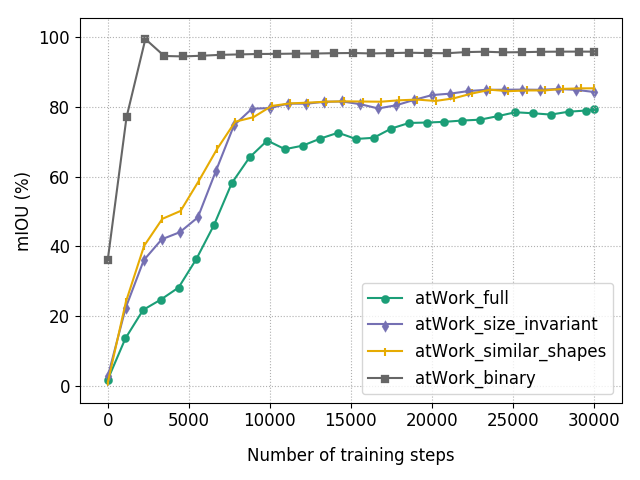
\includegraphics[width=1\linewidth]{images/mobi_4vars_white}
			\label{Fig:mobivarsb}
			\caption{}
		\end{subfigure}
		\begin{subfigure}{.5\textwidth}
			\centering
			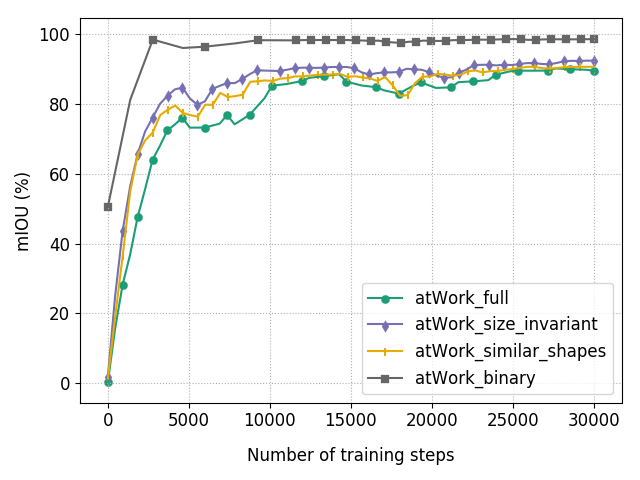
\includegraphics[width=1\linewidth]{images/xcep_4vars}
			\label{Fig:xcepvarsa}
			\caption{}
		\end{subfigure}
		\begin{subfigure}{.5\textwidth}
			\centering
			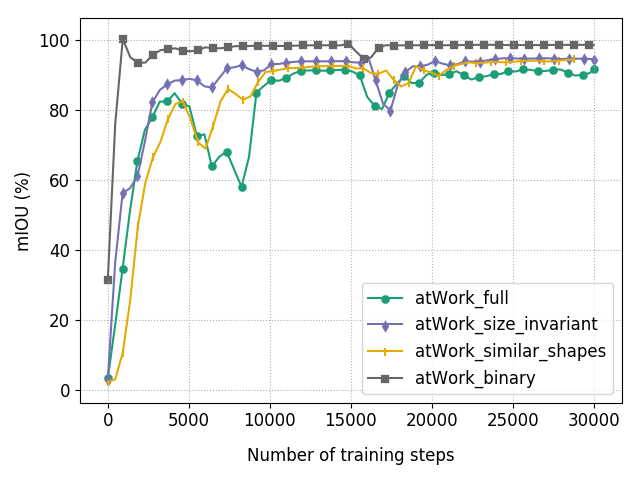
\includegraphics[width=1\linewidth]{images/xcep_4vars_white}
			\label{Fig:xcepvarsb}
			\caption{}
		\end{subfigure}
		\caption{mIOU of deeplabv3+ on the different dataset variants. (a) MobileNetv2 network backbone on variety of backgrounds dataset, (b) MobileNetv2 network backbone on white backgrounds dataset, (c) Xception network backbone on variety of backgrounds dataset, (d) Xception network backbone on white backgrounds dataset.}
		\label{Fig:vars}
	\end{figure}
	
	\begin{table}
	\centering
	\begin{tabular}{|c|c|c|c|c|c|c|c|}
	\hline 
	\multicolumn{ 1}{|l|}{\makecell{\textbf{Dataset variant}}} & \multicolumn{ 4}{l|}{\makecell{\textbf{mIOU in \%}}} \\ \cline{ 2- 5}
	\multicolumn{ 1}{|l|}{} & \multicolumn{ 2}{l|}{MobileNetv2 backbone} & \multicolumn{ 2}{l|}{Xception backbone} \\ \cline{ 2- 5}
	\multicolumn{ 1}{|l|}{} & VB & WB & VB & WB \\ \hline 
	atWork\_full & 77.47 & 79.26 & 89.63 & 91.59 \\ 
	\hline 
	atWork\_size\_invariant & 83.10 & 84.29 & 92.47 & 94.27 \\ 
	\hline 
	atWork\_similar\_shapes & 82.10 & 85.33 & 90.71 & 94.33 \\ 
	\hline 
	atWork\_binary & 96.06 & 95.83 & 98.68 & 98.47 \\ 
	\hline 
	\end{tabular}
	\caption{This table lists the mIOU obtained by deepLabv3+ with MobileNetv2 and Xception network backbones on 4 dataset variants of VB: variety of backgrounds dataset and WB: white backgrounds dataset.} 
	\label{Table:vars}
\end{table}

\section{Comparing deepLabv3+ backbones}

	\begin{itemize}
		\item \textbf{Objective}: The objective of this experiment is to compare the mIOUs obtained by deepLabv3+ with mobileNetv2 and Xception network backbones on each of the datasets and its variants.
		\item \textbf{Expected result}: The Xception network backbone is expected to obtain higher mIOU because of the higher number of learnable parameters in comparison with the mobileNet network backbone. In essence, the Xception network backbone has more "learning capacity" than the mobileNetv2 network backbone leading to the ability to learn a better decision boundary.
		\item \textbf{Inference from the results}: The results obtained are shown in Figure \ref{Fig:backbones}. Across all the dataset variants, the Xception network backbone achieves higher mIOU than the mobileNetv2 network backbone consistently. Another inference is that the models trained and validated on the white backgrounds dataset achieves slightly higher mIOU than corresponding models trained on the variety of backgrounds dataset. This could be because the model has to handle less variations in terms of backgrounds in the white backgrounds dataset as the backgrounds in this dataset are similar to each other.
	\end{itemize}

	\begin{figure}
		\begin{subfigure}{.5\textwidth}
			\centering
			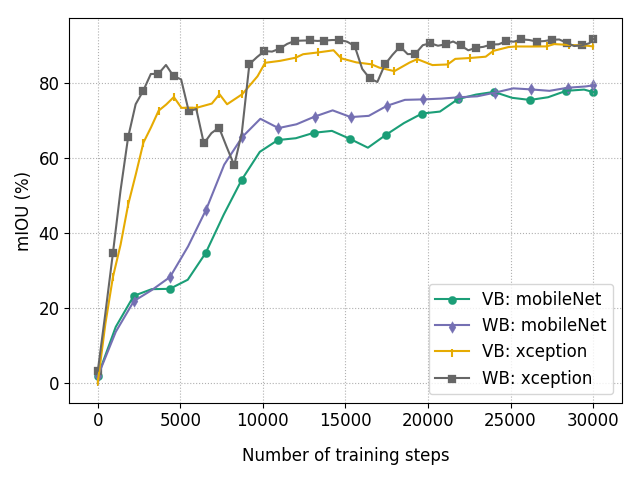
\includegraphics[width=1\linewidth]{images/mobxcep_full}
			\label{backbonesa}
			\caption{}
		\end{subfigure}
		\begin{subfigure}{.5\textwidth}
			\centering
			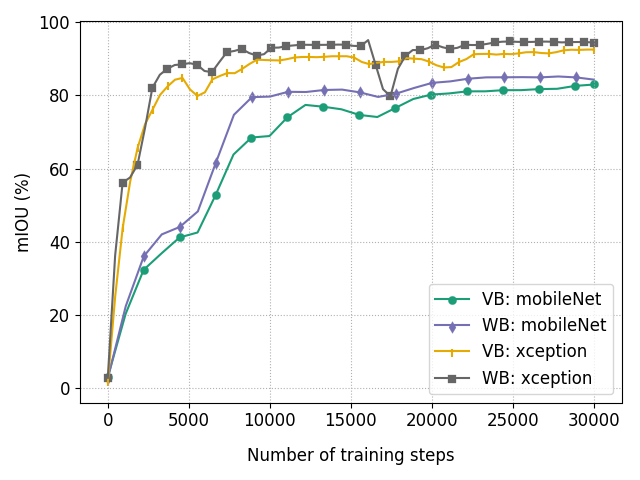
\includegraphics[width=1\linewidth]{images/mobxcep_size}
			\label{backbonesb}
			\caption{}
		\end{subfigure}
		\begin{subfigure}{.5\textwidth}
			\centering
			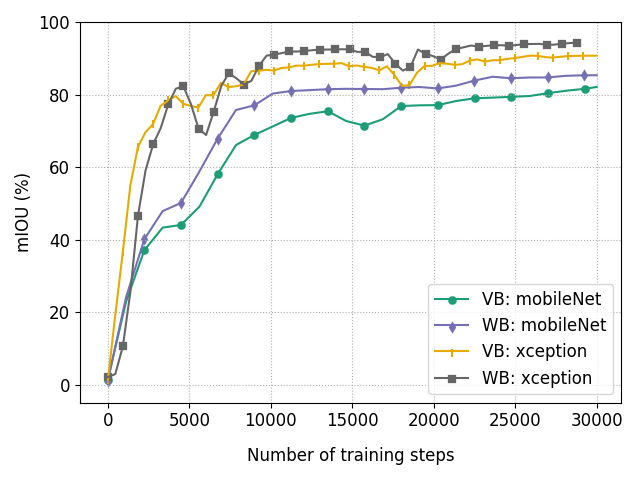
\includegraphics[width=1\linewidth]{images/mobxcep_shape}
			\label{backbonesc}
			\caption{}
		\end{subfigure}
		\begin{subfigure}{.5\textwidth}
			\centering
			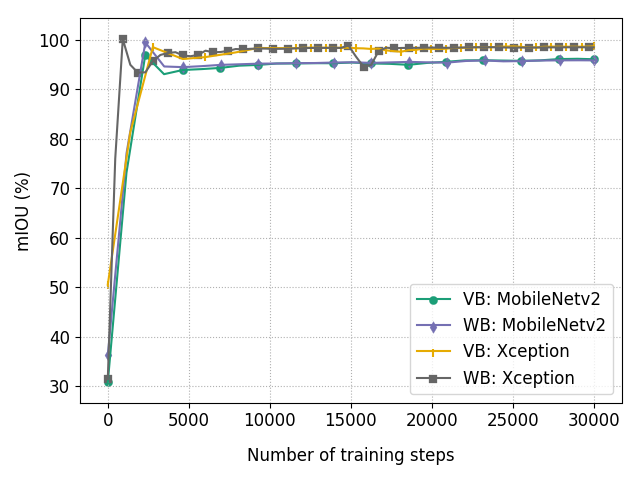
\includegraphics[width=1\linewidth]{images/mobxcep_binary}
			\label{backbonesd}
			\caption{}
		\end{subfigure}
		\caption{Comparison of mIOU obtained by deepLabv3+ using mobileNetv2 network backbone vs Xception network backbone on all 4 variants. VB denotes the variety of backgrounds dataset and WB denotes the white backgrounds dataset. The dataset variant is (a): atWork\_full, (b): atWork\_size\_invariant, (c): atWork\_similar\_shapes and (d): atWork\_binary.}
		\label{Fig:backbones}
	\end{figure}

\section{Training with different data}

	\begin{itemize}
		\item \textbf{Objective}: The objective of this experiment is to assess the effectiveness of the created artificial data. On this regards, starting from the same initial weights, deepLabv3+ with each of the two network backbones is trained on:
		\begin{itemize}
			\item[1] Entire training set of the variety of backgrounds dataset consisting of both real and artificial images.
			\item[2] Only the artificial images in the training set of variety of backgrounds dataset.
			\item[3] Entire training set of the white backgrounds dataset consisting of both real and artificial images.
			\item[4] Only the real training images.
		\end{itemize}
	The validation set only consists of the real validation images in order to consider only real world conditions.
		\item \textbf{Expected result}: Training with the entire training set of the variety of backgrounds dataset is expected to achieve the highest mIOU. This is based on the notion that the artificial images forces the segmentation model to learn features independent of the background. Also, the model is expected to have improved robustness towards varying object scales and occlusions. Training with just the real training images is also expected to perform well but second to the performance obtained with the entire variety of backgrounds training set. Training with white backgrounds dataset is expected to perform well except in cases where the background is not predominantly white. Training only with the artificial images is expected to perform the worst as it does not introduce the segmentation model to real world conditions.
		\item \textbf{Inference from the results}: From the results shown in Figure \ref{Fig:realval} and in Figure \ref{Fig:realvalxcep} it is evident that in all variants, training with just the real images achieves the best mIOU on the real validation set. This is in contrast to the notion that augmenting with artificial images improves mIOU. This apparent contrast begs to question the need for artificial images and states that they are not required. However, looking into the limitations of the real validation set could help reinstate the importance of the artificial images.
		\begin{itemize}
			\item[1] The real validation images only contain one object per image which in most images is clearly visible. There is no cases of occlusion or existance of multiple objects. 
			\item[2] The backgrounds in the real validation set is already seen in the training set. Only three different real backgrounds were used.
		\end{itemize}
		These two limitations exist in the real validation because of the need to reduce the labeling cost. Creating real world variations in terms of multiple objects per image and random occlusions is time consuming and also leads to increase in annotation time. Introducing varied backgrounds in real images is also time consuming. These limitations are addressed by the artificial images by placing objects at arbitrary scales in random locations on varied backgrounds.
		In addition to the existing limitations, the artificial images inherently impose a regularization effect on the training process. This can be attributed to the existence of many different backgrounds. On this regard, the existing L2 regularization weight decay term might need to be lowered to enable the model to better fit to the training data.
		\item \textbf{Suggestions to improve the experiment}: Adding a limited number of real validation images which have multiple objects and occlusions, reducing the value of L2 weight decay are two possible changes which can be introduced to arrive at a better inference. However, at this point in order to validate these speculations, model trained only on real data is validated on artificial data. \textbf{[result to be attached]} In this case, the mIOU obtained is only around 40 percent proving that this speculation could be further explored.
	\end{itemize}
	
	\begin{figure}
		\centering
		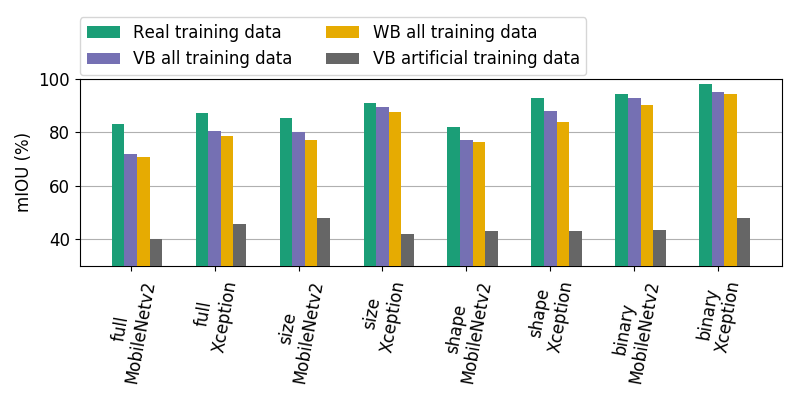
\includegraphics[width=1\linewidth]{images/real_val}
		\caption{This plot shows the mIOUs obtained when training deepLabv3+ on different training sets. "full" denotes the atWork\_full variant, "size" denotes the atWork\_size\_invariant variant, "shape" denotes the atWork\_similar\_shapes variant, "binary" denotes the atWork\_binary variant.}
		\label{Fig:realval}
	\end{figure}

\begin{table}
\centering
\begin{tabular}{|l|l|r|r|r|r|}
\hline
\multicolumn{ 1}{|l|}{\textbf{Dataset variant}} & \multicolumn{ 1}{l|}{\textbf{Backbone}} & \multicolumn{ 4}{l|}{\makecell{\textbf{mIOU in \%}}} \\ \cline{ 3- 6}
\multicolumn{ 1}{|l|}{} & \multicolumn{ 1}{l|}{} & \textbf{Real} & \makecell{\textbf{VB:} \\ \textbf{All}} & \makecell{\textbf{WB:} \\ \textbf{All}} & \makecell{\textbf{VB:} \\ \textbf{Artificial}} \\ \hline
\multicolumn{ 1}{|l|}{atWork\_full} & MobileNetv2 & 83.21 & 71.72 & 70.80 & 40.00 \\ \cline{ 2- 6}
\multicolumn{ 1}{|l|}{} & Xception & 87.03 & 80.26 & 78.42 & 45.67 \\ \hline
\multicolumn{ 1}{|l|}{atWork\_size\_invariant} & MobileNetv2 & 85.01 & 80.08 & 77.12 & 47.76 \\ \cline{ 2- 6}
\multicolumn{ 1}{|l|}{} & Xception & 90.84 & 89.58 & 87.67 & 41.58 \\ \hline
\multicolumn{ 1}{|l|}{atWork\_similar\_shapes} & MobileNetv2 & 79.83 & 77.33 & 76.47 & 43.31 \\ \cline{ 2- 6}
\multicolumn{ 1}{|l|}{} & Xception & 92.85 & 87.76 & 83.58 & 43.32 \\ \hline
\multicolumn{ 1}{|l|}{atWork\_binary} & MobileNetv2 & 94.33 & 93.01 & 90.17 & 43.29 \\ \cline{ 2- 6}
\multicolumn{ 1}{|l|}{} & Xception & 98.19 & 95.21 & 94.31 & 47.91 \\ \hline
\end{tabular}
\caption{This table summarizes the mIOUs obtained when training with different training data and validating on the real validation data. "Real" denotes real training data, "VB: All" denotes real and artificial data of the variety of backgrounds dataset, "WB: All" denotes real and artificial data of the white backgrounds dataset, "VB: Artificial" denotes artificial data of the variety of backgrounds dataset.}
\label{Table:realval}
\end{table}

\section{Comparing individual classes}

	\subsection{Confusion matrix}
		\begin{itemize}
			\item \textbf{Objective}: The objective of this section is to analyze the deepLabv3+ models inability to distinguish between different objects. 
			\item \textbf{Expected result}: The variants with higher number of classes is expected to have more non leading diagonal terms in the confusion matrix. This is based on the belief that the segmentation model would face difficulties distinguishing objects very similar to each other. This problem is expected to be alleviated by the atWork\_size\_invariant and atWork\_similar\_shapes variants. On the atWork\_binary variant, there is a possibility that a certain percentage of foreground pixels are confused with background.
			\item \textbf{Inference from the results}: On all the confusion matrices, the leading diagonal elements have highest values in each row. This is expected and suggests that the model correctly classifies a majority of pixels in each class. Notably, the objects confused with each other are either similar in terms of color or shape. For instance, around 10 percent of m30 is confused as m20. This is reasonable as the objects are similar in shape and only differ in size. The difference in size cannot be picked up by the model as no consistent information regarding the object size is available in the dataset. 41.18 percent of pixels in distance tube are confused with background. This could be because the number of pixels occupied by distance tube in the dataset is small in comparison to the other objects.
			Confusions between objects has reduced on the atWork\_size\_invariant and atWork\_similar\_shapes dataset in comparison to the atWork\_full variant. This can be attributed to the combining of similar objects to one class. The confusion between motor and m20\_100 and the confusion between motor and r20 needs to be addressed.
		\end{itemize}

		\begin{figure}
			\begin{subfigure}{1\textwidth}
				\centering
				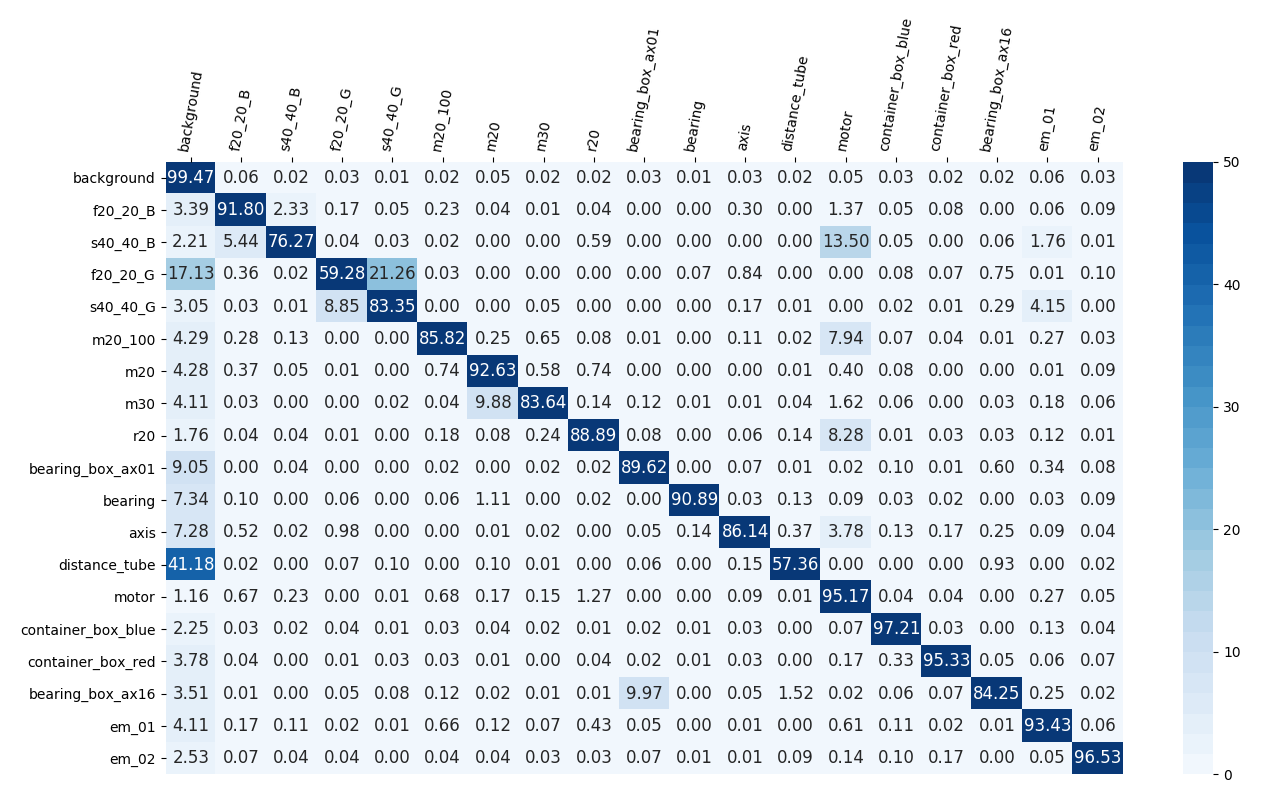
\includegraphics[width=0.8\linewidth]{images/cm_full}
				\caption{}
			\end{subfigure}
			\begin{subfigure}{1\textwidth}
				\centering
				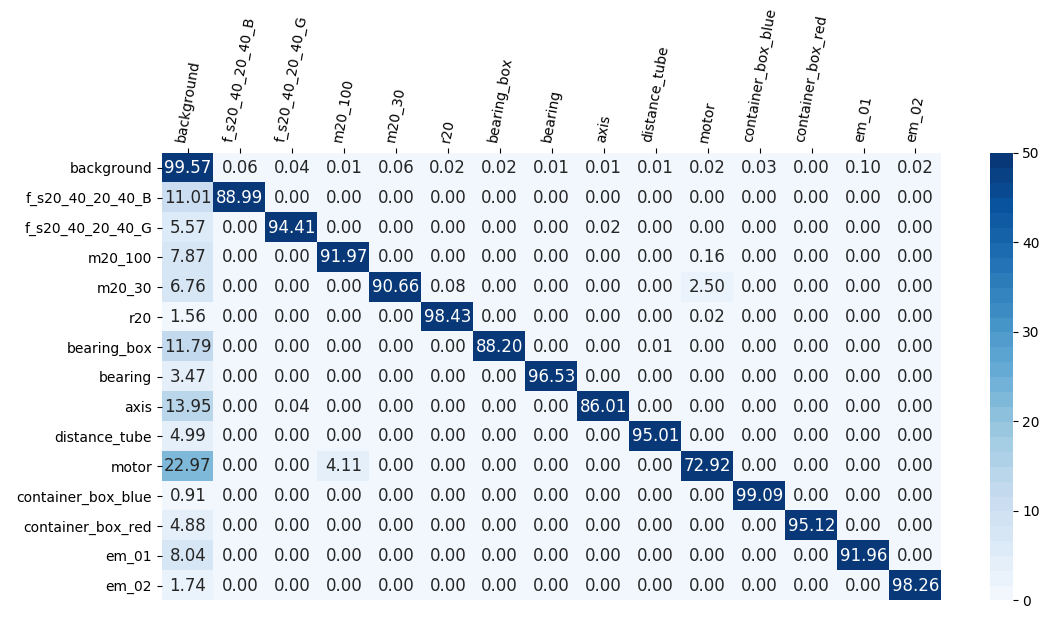
\includegraphics[width=0.7\linewidth]{images/cm_size}
				\caption{}
			\end{subfigure}
			\begin{subfigure}{.6\textwidth}
				\centering
				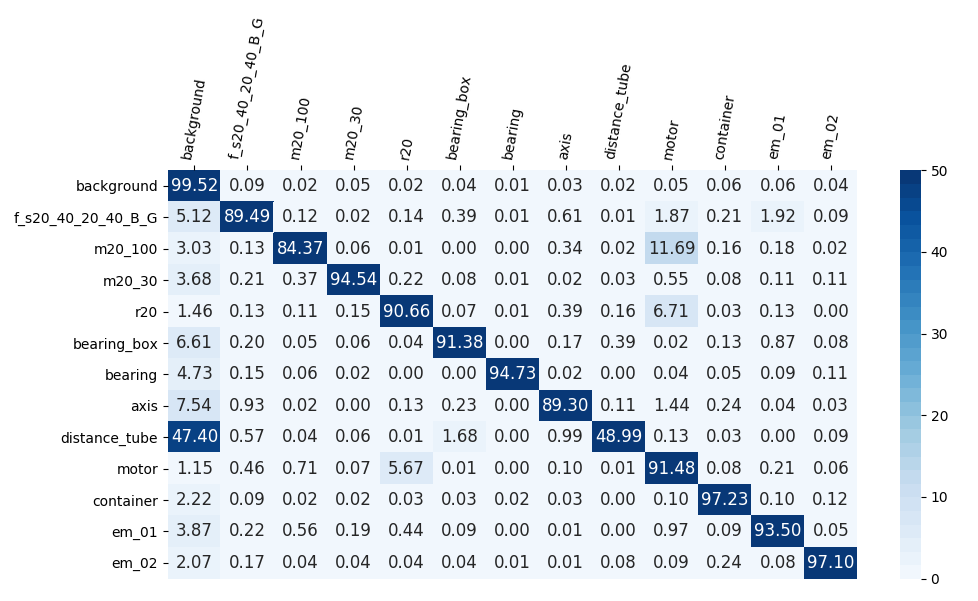
\includegraphics[width=0.9\linewidth]{images/cm_shape}
				\caption{}
			\end{subfigure}
			\begin{subfigure}{.3\textwidth}
				\centering
				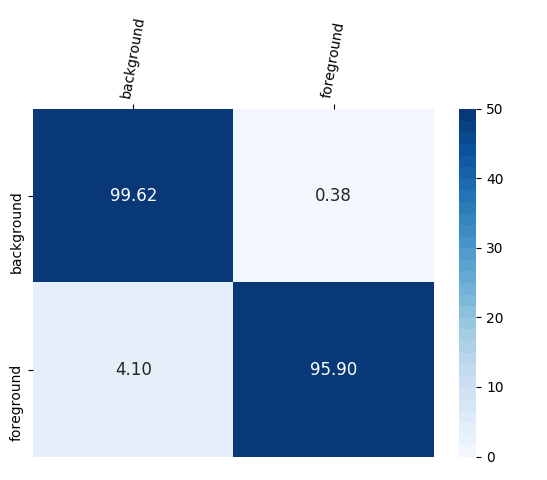
\includegraphics[width=0.9\linewidth]{images/cm_binary}
				\caption{}
			\end{subfigure}
			\caption{Confusion matrix of deepLabv3+ with mobileNet backbone based on number of classified pixels on all 4 variants of the variety of backgrounds dataset. The number of pixels in each row is normalized by the total number of pixels in the row. (a): atWork\_full variant, (b): atWork\_size\_invariant, (c): atWork\_similar\_shapes and (d): atWork\_binary.}
			\label{Fig:cm}
		\end{figure}
	
	\subsection{Class IOUs}	
		\begin{itemize}
			\item \textbf{Objective}: The objective of this experiment is to look for a relationship between the individual class IOUs and the percentage of pixels occupied by each class in the dataset. 
			\item \textbf{Expected result}: With increase in percentage of pixels, the class IOU is expected to increase. This is based on the notion that the segmentation model gives preference to objects which dominate the dataset. 
			\item \textbf{Inference from the results}: For each class, the mean over 30000 training steps of class IOU is calculated. Both the percentage of pixels and the class IOU is normalized with respect to the maximum value out of all objects. The classes are arranged in increasing order of percentage of pixels. The plots are shown in \ref{Fig:clsiou}. From the lower histogram plot for atWork\_full variant shown in \ref{Fig:clsioua}, the class IOUs denoted by the green bars do not seem to show an increasing trend. However, when every 3 classes starting from class distance\_tube are combined and plotted separately, (shown in the upper graph of \ref{Fig:clsioua}). Similar observations can be made for the other two variants as shown in \ref{Fig:clsioub} and \ref{Fig:clsiouc}. 
			Another interesting result is that the segmentation model seems to learn the object "bearing" well despite the fact that the object only occupies few pixels in the dataset. This could be because of the distinct black ring in between two silver rings present in the bearing. This pattern seems unique and the model probably picks up this pattern with ease.
		\end{itemize}
	
		\begin{figure}[!htb]
			\begin{subfigure}{1\textwidth}
				\centering
				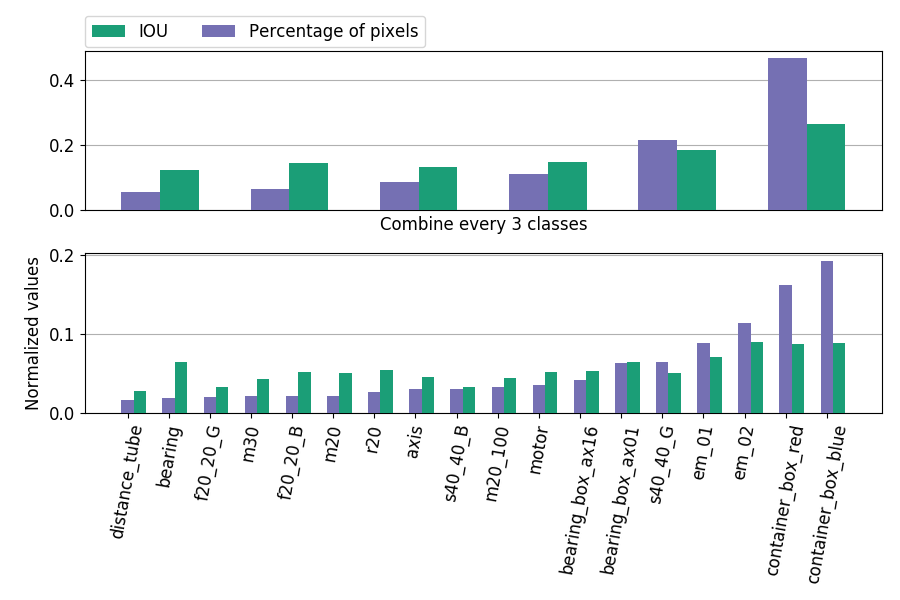
\includegraphics[width=1\linewidth]{images/cls_iou_full}
				\caption{}
				\label{Fig:clsioua}
			\end{subfigure}
			\begin{subfigure}{.5\textwidth}
				\centering
				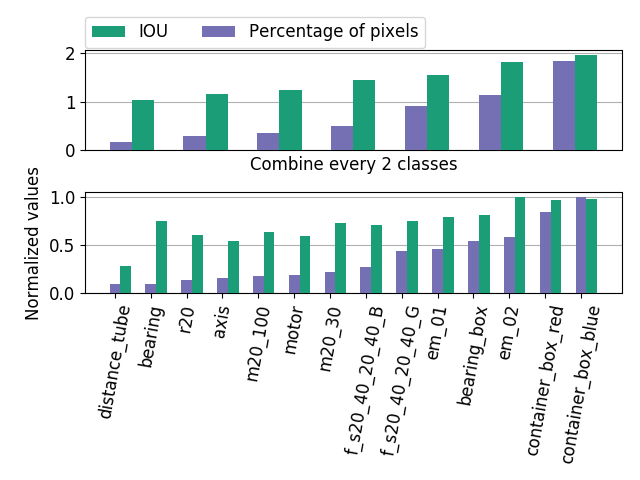
\includegraphics[width=1\linewidth]{images/cls_iou_size}
				\caption{}
				\label{Fig:clsioub}
			\end{subfigure}
			\begin{subfigure}{.5\textwidth}
				\centering
				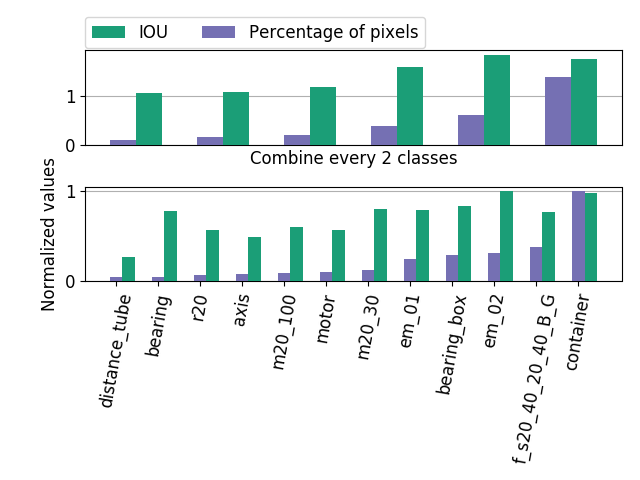
\includegraphics[width=1\linewidth]{images/cls_iou_shape}
				\caption{}
				\label{Fig:clsiouc}
			\end{subfigure}
			\caption{Individual class IOUs achieved by deepLabv3+ with mobileNet backbone is plotted with the percentage of pixels occupied on all 4 variants of the variety of backgrounds dataset. The number of pixels in each row is normalized by the total number of pixels in the row. (a): atWork\_full variant, (b): atWork\_size\_invariant, and (c): atWork\_similar\_shapes.}
			\label{Fig:clsiou}
		\end{figure}

\section{Comparing learning rate policies}
	
	\begin{itemize}
		\item \textbf{Objective}: The objective of this experiment is to compare the cosine restarts \textbf{[needs reference]} learning rate policy with the poly learning rate policy used by deepLabv3+.
		\item \textbf{Expected result}: Either of the two learning rate policies is expected to result in better Mean IOU.
		\item \textbf{Inference from the results}: DeepLabv3+ with mobileNet backbone is used for this experiment. Evidently, the cosine restart learning rate policy leads to slightly better Mean IOU on both the atWork\_binary and the atWork\_size\_invariant variants.
	\end{itemize}
	
	\begin{figure}
		\begin{subfigure}{.3\textwidth}
			\centering
			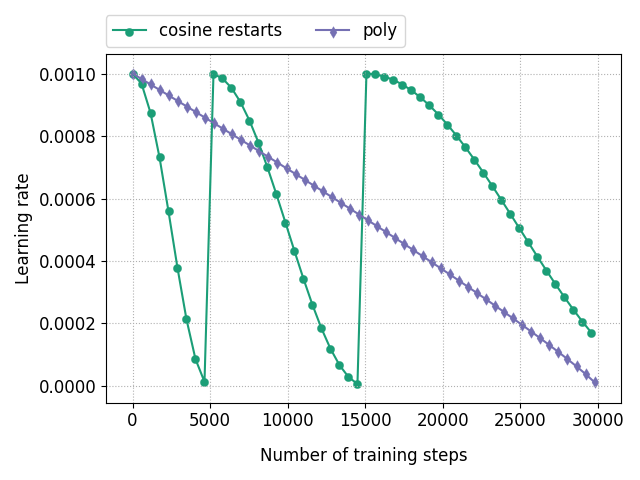
\includegraphics[width=1\linewidth]{images/lr_train_bin}
			\caption{}
		\end{subfigure}
		\begin{subfigure}{.3\textwidth}
			\centering
			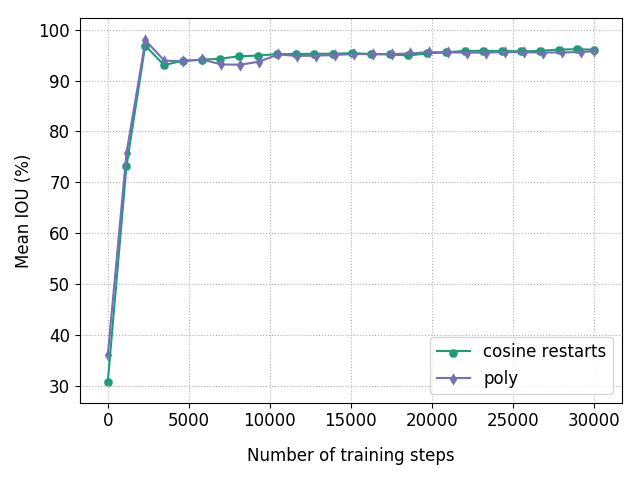
\includegraphics[width=1\linewidth]{images/lr_binary}
			\caption{}
		\end{subfigure}
		\begin{subfigure}{.3\textwidth}
			\centering
			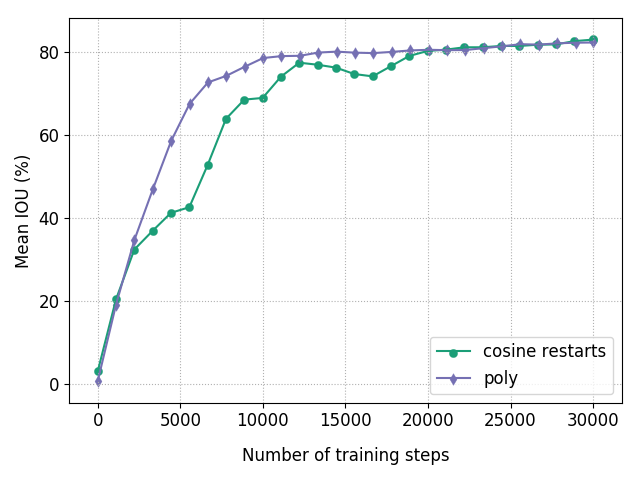
\includegraphics[width=1\linewidth]{images/lr_size}
			\caption{}
		\end{subfigure}
		\caption{Learning rate decay with two different policies 1. cosine restarts and 2. poly is compared. (a): learning rate over 30000 steps with the two decay policies. (b): Mean IOU on the validation set of atWork\_binary variant is 96.06 \% with cosine restarts and 95.75 \% with poly. (c): Mean IOU on the validation set of atWork\_size\_invariant variant is 83.1 \% with cosine restarts and 82.24 \% with poly.}
		\label{Fig:lr}
	\end{figure}

\section{Effects of class balancing}

% About attempt to counter failure in distance tube.
	\begin{itemize}
		\item \textbf{Objective}: The objective of this experiment is to prevent the deepLabv3+ model from giving preference to dominant classes in the dataset. A weight coefficient is determined for each class based on the percentage of pixels occupied by the class in the dataset. These weight coefficients are multiplied with the loss term of the corresponding class in the loss function.
		\item \textbf{Expected result}: The model is expected to achieve similar class IOUs on all the objects. The overall Mean IOU is also expected to be comparable to the Mean IOU obtained without class balancing.
		\item \textbf{Inference from the results}: 
	\end{itemize}

\section{Effects of quantizing the inference graph}
	
	\begin{itemize}
		\item \textbf{Objective}: The objective of this experiment is to compare a model with floating point weights and the corresponding model with fixed point weights in terms of Mean IOU, occupied disk memory and inference time.
		\item \textbf{Expected result}:
		\item \textbf{Inference from the results}:
	\end{itemize}

	\begin{figure}
		\begin{subfigure}{.5\textwidth}
			\centering
			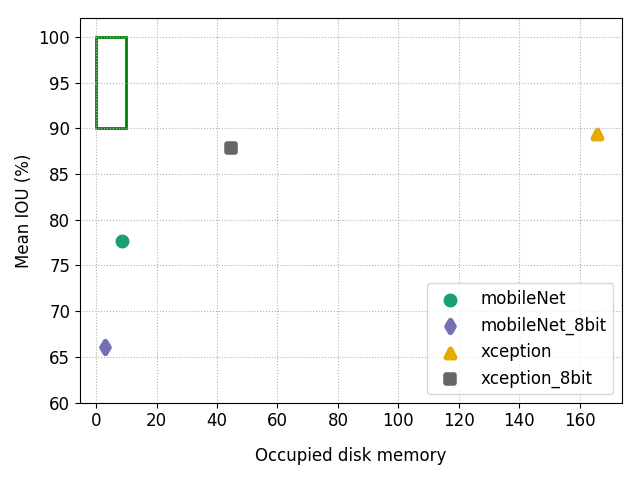
\includegraphics[width=1\linewidth]{images/q_mem_v_full}
		\end{subfigure}
		\begin{subfigure}{.5\textwidth}
			\centering
			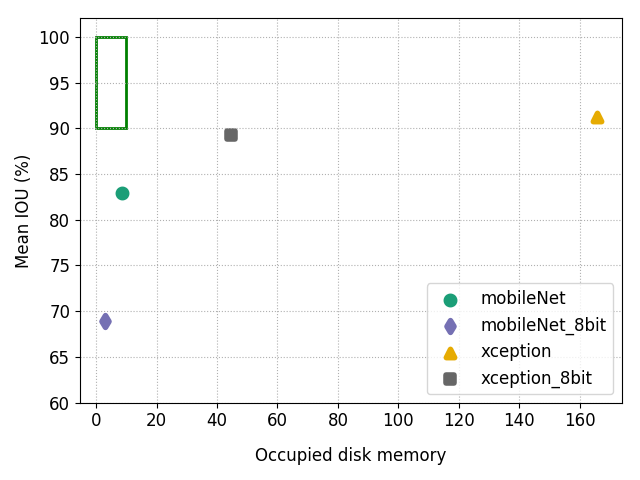
\includegraphics[width=1\linewidth]{images/q_mem_v_size}
		\end{subfigure}
		\begin{subfigure}{.5\textwidth}
			\centering
			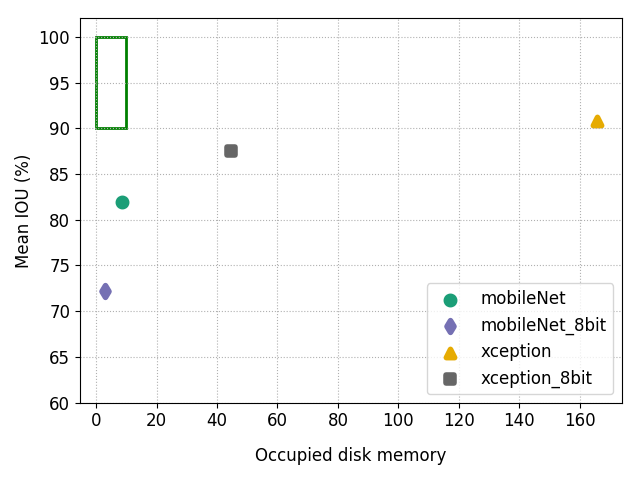
\includegraphics[width=1\linewidth]{images/q_mem_v_shape}
		\end{subfigure}
		\begin{subfigure}{.5\textwidth}
			\centering
			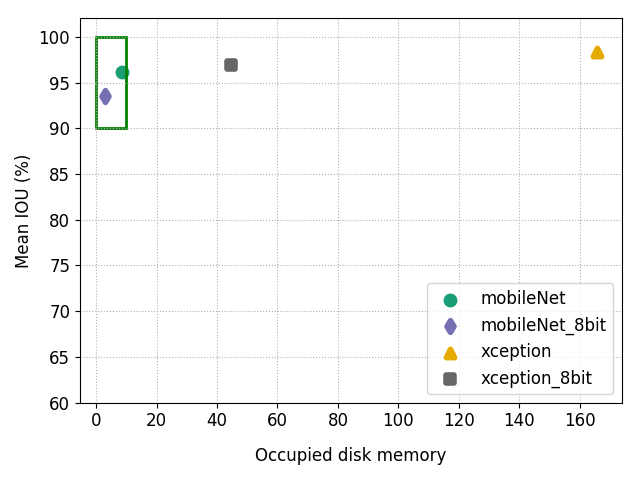
\includegraphics[width=1\linewidth]{images/q_mem_v_bin}
		\end{subfigure}
		\caption{.}
		\label{Fig:quant}
	\end{figure}

\section{Transfer learning}

	\begin{itemize}
		\item \textbf{Objective}:
		\item \textbf{Expected result}:
		\item \textbf{Inference from the results}: Size invariant;mobileNet: PASCAL VOC 2012 = 83.1, mobileNet: atWork\_binary = 83.26, xception: PASCAL VOC 2012 = 91.19, xception: atWork\_binary = 92.14...Similar shapes;mobileNet: PASCAL VOC 2012 = 82.1, mobileNet: atWork\_binary = 82.8, xception: PASCAL VOC 2012 = 90.81, xception: atWork\_binary = 92.15...Full;mobileNet: PASCAL VOC 2012 = 77.47, mobileNet: atWork\_binary = 77.73, xception: PASCAL VOC 2012 = 89.38, xception: atWork\_binary = 90.64
	\end{itemize}
	
	
	\begin{figure}
		\begin{subfigure}{.3\textwidth}
			\centering
			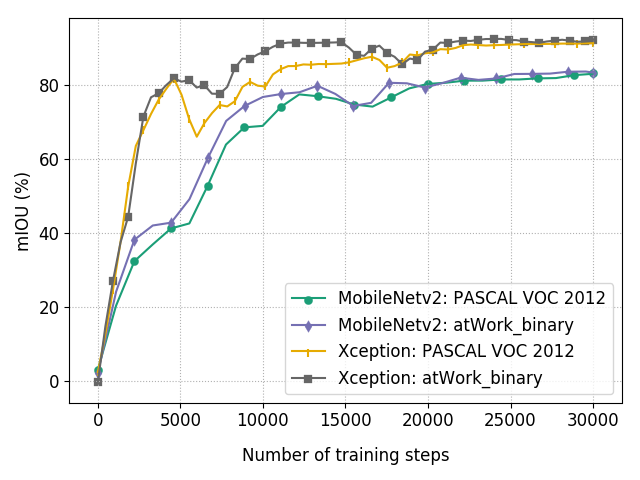
\includegraphics[width=1\linewidth]{images/transfer_size}
			\caption{}
		\end{subfigure}
		\begin{subfigure}{.3\textwidth}
			\centering
			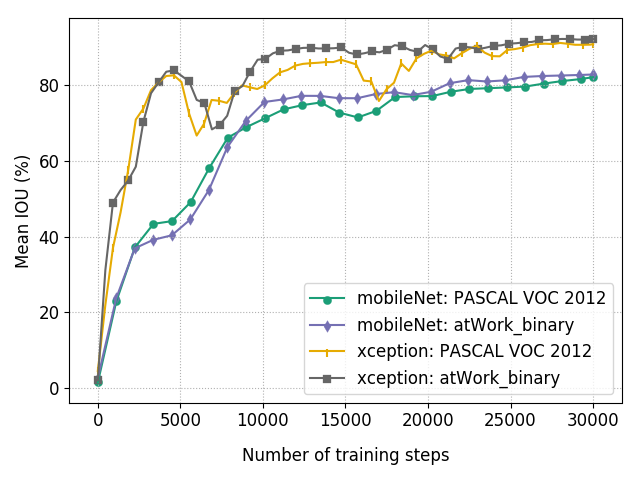
\includegraphics[width=1\linewidth]{images/transfer_shape}
			\caption{}
		\end{subfigure}
		\begin{subfigure}{.3\textwidth}
			\centering
			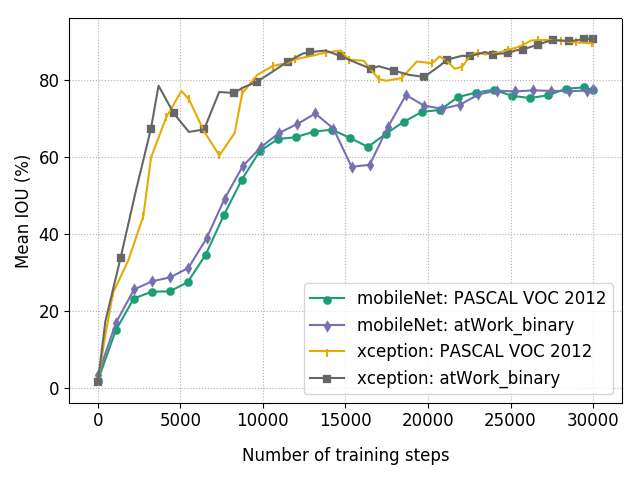
\includegraphics[width=1\linewidth]{images/transfer_full}
			\caption{}
		\end{subfigure}
		\caption{Mean IOU for 30,000 training steps obtained on three variants by deepLabv3+ with xception and mobileNetv2 as network backbones when pretrained on either PASCAL VOC 2012 dataset or atWork\_binary variant. As expected, pretrained weights from atWork\_binary variant leads to a better Mean IOU. The figures show the results on variants of the variety of backgrounds dataset: (a) atWork\_size\_invariant, (b) atWork\_similar\_shapes, (c) atWork\_full.}
		\label{Fig:transfer}
	\end{figure}

